\documentclass[12pt]{article}
\usepackage[margin=1.0in]{geometry}
\usepackage[utf8]{inputenc}
\usepackage[T1]{fontenc}
\usepackage{lmodern}
\usepackage[spanish]{babel}
\usepackage{amsmath}
\usepackage{graphicx}

\title{Response to the referee}

\begin{document}

\date{}
\maketitle

Dear referee the main changes in our paper are that we do find 

\section{Global Comments}

\subsection{Variation with the viewing angle}

The problematic of anisotropy is only studied from Sect3.4, the former sections consider global quantities (spectral shapes, escape fractions, etc...). This is ok only if there is NO anisotropy induced by rotation, which is not obvious, a priori. You should make it clear from the beginning, telling that you will investigate anisotropy at the end of the paper only, because you checked that lya properties are isotropic, at least in the range of parameters that you investigated so far.\\


\textbf{ We have decide to study in this paper the case in which there is No anisotropy. The part concerning the off-center emission is going to be presented in a later study\\}

As explained in sect 3.4, rotation kills the spherical symmetry of your problem, and the rotation axis defines a preferential direction. We could expect some variation of the emerging flux, the lyman-alpha escape fraction, and the spectral shape, with viewing angle. From Fig8, it seems that the flux is the same in all directions for spherical distributions of sources. This important result is not enough emphasized.\\

\textbf{We do not find the flux variation with the viewing angle and now as highlighted in the new text we emphasize more this new result, also we made a new plot Figure 5 in the paper, showing this results for both distributions (homogeneous/central) and for optical depth $\tau_{H}=10^{5}$ we choose these models because this are the ones 
that are more sensitive to rotation.}\\

Do you see any difference in the spectral shape with viewing angle? To illustrate this point, it would be interesting to build a 2D plot as you did on Fig 5, but replace Nb scat in ordinates by the viewing angle $\mu$. We could immediatly see if there is an evolution of the shape with viewing angle or not. If you find NO evolution of the Lya shape with viewing angle, I think that it is an interesting counter-intuitive result, that you should advertise more.\\

\textbf{Thanks very much for this recommendation we made this new plot and we do find variations in the morphology of the line due to variations in the viewing angle. We have restructure the paper this new plots now correspond to figure 2 \& 3 in the paper.  Also we emphasize this results in the results, discussion and conclusion sections.\\}

What about the variation of lya escape fraction with viewing angle ? I propose that in the beginning of Sect.3 Results, you first emphasize that, maybe counter-intuitively, you did not find any variation of the Lya properties with viewing angle, so you will present first angle average lya properties, and you will come back to the anisotropy problematic only at the end on the paper.\\

\textbf{As escape fraction depends on the number of scatterings and this is invariant for different viewing angles the escape fraction does not change with the viewing angle. (MAKE A PLOT AND EXPLAIN THIS BETTER)
}


\section*{Outflow + Rotation}

We want to study the pure effect of rotation on the spectra, off course it would
be interesting to study the effect of rotation on systems with outflows, this paper
is under preparation by M.C Remolina-Gutierrez et al.  

\section*{Details}

\subsection*{Introduction}

With Orsi et al 2012, please cite also Garel et al 2012. With Zheng \& Wallace 2013, please cite also Behrens et al 2014.\\

\textit{This changes were performed.}
\subsection*{Fig.1}

I guess that the spectra presented in Fig1 are integrated over all directions, right ? You should describe explicitly how you build them. You could skip the x notation in absciss, as it is not used in the discussion, whereas the velocity is used to compare to FWHM, on Fig2.\\

\textbf{Now this figure is the Fig.4 in the paper. what we did was to fix a viewing angle in this case $\theta= \pi/2$ and make the histogram of the photons frequency.}

\begin{itemize}
\item Description about how we build Fig.1 (Done)
\item Fig 1. remove x notation (Done)
\end{itemize}

\subsection*{Fig.2}

Fig.2 Can you explain how you measure the FWHM of a double-peaked profile ? Do you fit it with a gaussian ?


We don't fit a gaussian, we interpolate points to the line profile and then  we measure the width by finding
the closest points to the half maximum in our histogram.

\subsection*{Fig.3}

Do you have an idea why the (central source, intermediate optical depth) case with Vmax=300 has a single plateau instead of 2 peaks ? Do you find this with the two codes ?


\subsection*{Fig4 and 6}

This is a surprising result that the number of scatterings (escape fraction) stays constant as the rotation velocity increases, for a central source, whereas the global spectral shape is altered. Did you try with higher/extreme values of Vmax (=1000 km/s, even if not physically motivated) ? Do you believe that the number of scatterings decreases with very high values, or that it is independant of the rotation velocity ? Is the escape fraction from a dusty rotating cloud with central source independant of the rotation velocity ?

\subsection*{Fig5}
This is a very nice figure ! Looking at the top right panel, with its “photosphere”, I’m surprised that the distribution of Nscatt is bipolar, I would have expected a smooth transition between the 2 regimes. Do you have a physical explanation why photons escape after either (less than 10) or (more than 1000) scatterings, and none escape with 100 scatt ? To test the ’photosphere’ assumption, you could also do the radiation transfer in a cloud with the distribution of sources only in an inner sphere, and another experienment with sources only in an outer shell. If I understood corectly, you would expect thant the bottom spot on the top right panel is made of photons from the outer shell, and the uppper spot from photons emitted inside the cloud.

\begin{figure}
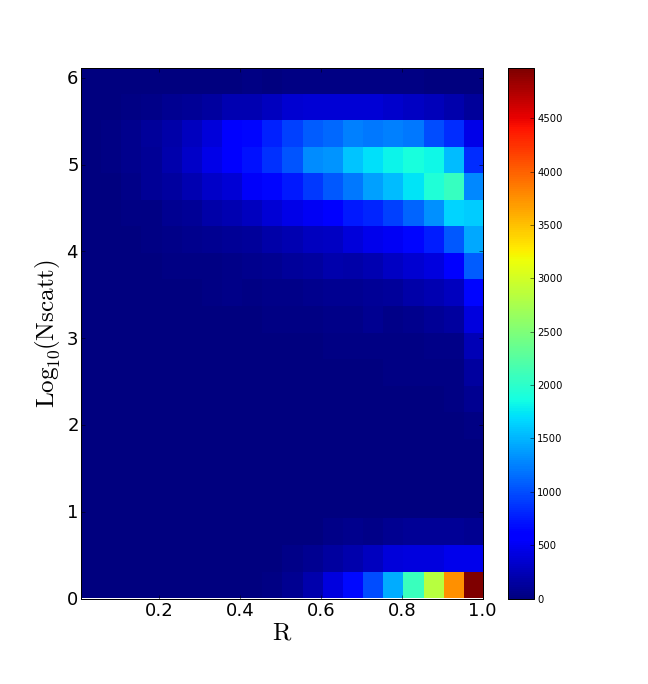
\includegraphics[scale=0.4]{Histogram2dNscattVSRadius.png}
\end{figure}


\subsection*{End of paragraph 3.3}

One sentence is not clear : we see that the escape fraction does not increase significantly from $\tau$ = 105 to $\tau = 10^{6}$. This counter-intuitive result.... It sounds like you were expecting a strong increase... A decrease is expected from $\tau$ = 105 to $\tau$ = 106, not an increase, but indeed on the graphe we can see an unexpected (small) increase. I do not understand the explanation for this behaviour.
(Mark)

\subsection*{Fig8}


Referred to as Figure 7 in the text (paragraph 3.4). To my mind, this figure illustrates the main result of your study, it has to be more demonstrative. On this figure, the numerical noise seems very big compare to the small number of bins, bigger than on the spectra from Fig1, how is it possible ? Could you re-do this figure with more photons, maybe with more bins ? Could you plot an histogram instead of broken lines, to ease the reading ? In the text, you write anisotropy induced by rotation is at the 3$\%$ level, how do to estimate this number? I think that the noise is at $3\%$ level, and the distribution is compatible with ’flat’. In the corresponding text, you first say that $F(\mu)$ does not depend on Vmax. Again, if real, this is an important result, that you must advertise more. Please show it on this Fig, by comparing F(μ) without rotation (in red, for example) to the other distributions that you get with different values of Vmax. Then, you mention that for high optical depth values, $F(\mu)$ (not the variations of $\mu$) can vary up to $15\%$. First, what do you call high optical depth ? your highest setup is τ = 107, not extremely high for lyman alpha ”standards’, corresponding to NHI ∼ 1020 cm−2. So, if you see a trend with optical depth, I encourage you to check higher optical depth regimes, corresponding better to galaxy scales. If you can probe that anisotropy induced by rotation is rising with optical depth, this would be an interesting result.
If higher optical depth regimes lead to anisotropic escape, could you check the effet of anisotropy on the lya spectral shape ?



\end{document}